% Fig. 2 评估协议与增强来源总览（TikZ 示意图）；编译：pdflatex fig2_protocol.tex
\documentclass[10pt]{standalone}
% 全部论文图共用的样式（颜色固定跟随来源；字号按 elsarticle 正文 10pt 设定）
% 颜色来自经过色觉校验的分类调色板，顺序固定：
%   类别权重 = 1 蓝，ROS = 2 橙，SMOTE = 3 青，Qwen = 4 黄，Llama = 5 品红；不增强 = 中性灰
\usepackage{pgfplots}
\usepgfplotslibrary{groupplots}
\pgfplotsset{compat=1.18}
\usetikzlibrary{plotmarks,calc,patterns,arrows.meta,positioning,shapes.geometric,fit,backgrounds}
\definecolor{cCW}{HTML}{2A78D6}
\definecolor{cROS}{HTML}{EB6834}
\definecolor{cSMOTE}{HTML}{1BAF7A}
\definecolor{cQWEN}{HTML}{EDA100}
\definecolor{cLLAMA}{HTML}{E87BA4}
\definecolor{cNONE}{HTML}{52514E}
\definecolor{cGRID}{HTML}{E4E3DF}
\definecolor{cAXIS}{HTML}{8A8984}
\definecolor{cTEXT}{HTML}{2B2A28}
\pgfplotsset{
  paper/.style={
    font=\footnotesize, color=cTEXT,
    axis line style={cAXIS, line width=0.4pt},
    tick style={cAXIS, line width=0.4pt},
    major tick length=2pt,
    grid style={cGRID, line width=0.4pt},
    ymajorgrids,
    tick label style={font=\scriptsize},
    label style={font=\footnotesize},
    title style={font=\footnotesize\bfseries, yshift=-2pt},
    legend style={font=\scriptsize, draw=none, fill=none, /tikz/every even column/.append style={column sep=8pt}},
    legend cell align=left,
  },
  errbar/.style={error bars/.cd, y dir=both, y explicit,
    error bar style={line width=0.5pt, cTEXT!75}, error mark options={rotate=90, mark size=1.4pt, line width=0.5pt, cTEXT!75}},
}

\begin{document}
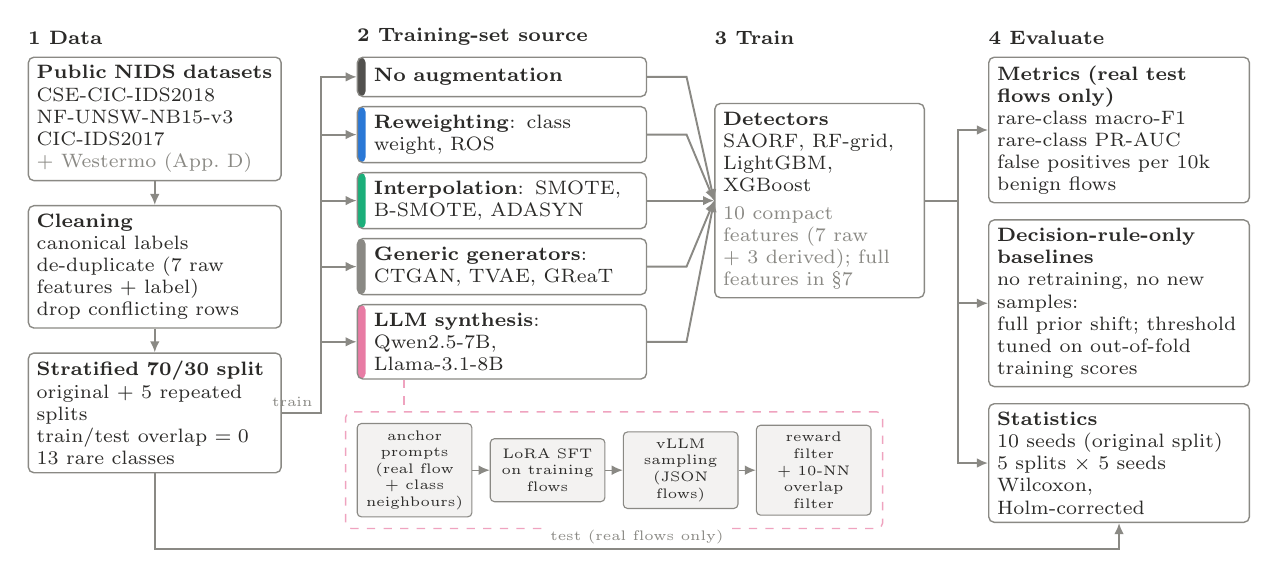
\begin{tikzpicture}[
  font=\scriptsize, color=cTEXT,
  every node/.append style={execute at begin node={\hyphenpenalty=10000\exhyphenpenalty=10000}},
  box/.style={draw=cAXIS, line width=0.5pt, rounded corners=2pt, fill=white, align=left, inner sep=3pt, text width=#1},
  box/.default=3.0cm,
  src/.style={box=3.25cm, minimum height=0.5cm, inner xsep=6pt,
    path picture={\fill[#1] (path picture bounding box.north west) rectangle ([xshift=3pt]path picture bounding box.south west);}},
  head/.style={font=\scriptsize\bfseries, anchor=south west, inner sep=0pt},
  arr/.style={-{Latex[length=4pt, width=3.5pt]}, cAXIS, line width=0.7pt},
  stp/.style={draw=cAXIS, line width=0.4pt, rounded corners=1.5pt, fill=cGRID!45, align=center, inner sep=2.5pt,
    text width=1.28cm, minimum height=0.8cm, font=\tiny},
  lab/.style={font=\tiny, cAXIS, inner sep=1.5pt, fill=white},
]
% ------------------------------------------------ 列 1：数据
\node[box] (data) at (0,0) {\textbf{Public NIDS datasets}\\CSE-CIC-IDS2018\\NF-UNSW-NB15-v3\\CIC-IDS2017\\{\color{cAXIS}+ Westermo (App.~D)}};
\node[box, below=0.3cm of data] (clean) {\textbf{Cleaning}\\canonical labels\\de-duplicate (7 raw features + label)\\drop conflicting rows};
\node[box, below=0.3cm of clean] (split) {\textbf{Stratified 70/30 split}\\original + 5 repeated splits\\train/test overlap $=0$\\13 rare classes};
\draw[arr] (data) -- (clean);
\draw[arr] (clean) -- (split);
\node[head] at ([yshift=4pt]data.north west) {1\,\,Data};
% ------------------------------------------------ 列 2：训练集来源
\node[src=cNONE, anchor=north west] (s0) at ([xshift=0.95cm]data.north east) {\textbf{No augmentation}};
\node[src=cCW, below=0.11cm of s0] (s1) {\textbf{Reweighting}: class weight, ROS};
\node[src=cSMOTE, below=0.11cm of s1] (s2) {\textbf{Interpolation}: SMOTE, B-SMOTE, ADASYN};
\node[src=cAXIS, below=0.11cm of s2] (s3) {\textbf{Generic generators}: CTGAN, TVAE, GReaT};
\node[src=cLLAMA, below=0.11cm of s3] (s4) {\textbf{LLM synthesis}: Qwen2.5-7B, Llama-3.1-8B};
\node[head] at ([yshift=4pt]s0.north west) {2\,\,Training-set source};
% 训练集 -> 各来源（总线）
\coordinate (bus) at ([xshift=-0.45cm]s0.west);
\draw[arr] (split.east) -- ([xshift=-0.45cm]split.east -| s0.west) |- (s0.west);
\node[font=\tiny, cAXIS, anchor=south east, inner sep=1pt] at ([xshift=-2pt,yshift=1pt]bus |- split.east) {train};
\foreach \s in {s1,s2,s3,s4} \draw[arr] (bus |- \s.west) -- (\s.west);
% ------------------------------------------------ 列 3：检测器
\node[box=2.45cm, anchor=west] (det) at ([xshift=0.85cm]s2.east) {\textbf{Detectors}\\SAORF, RF-grid, LightGBM, XGBoost\\[2pt]{\color{cAXIS}10 compact features (7 raw + 3 derived); full features in \S7}};
\node[head] at ([yshift=4pt]det.north west |- s0.north) {3\,\,Train};
\foreach \s in {s0,s1,s2,s3,s4} \draw[arr] (\s.east) -- ([xshift=-0.35cm]det.west |- \s.east) -- (det.west);
% ------------------------------------------------ 列 4：评估
\node[box=3.1cm, anchor=north west] (eval) at ([xshift=0.8cm]det.east |- s0.north) {\textbf{Metrics (real test flows only)}\\rare-class macro-F1\\rare-class PR-AUC\\false positives per 10k benign flows};
\node[box=3.1cm, below=0.2cm of eval] (base) {\textbf{Decision-rule-only baselines}\\no retraining, no new samples:\\full prior shift; threshold tuned on out-of-fold training scores};
\node[box=3.1cm, below=0.2cm of base] (stat) {\textbf{Statistics}\\10 seeds (original split)\\5 splits $\times$ 5 seeds\\Wilcoxon, Holm-corrected};
\node[head] at ([yshift=4pt]eval.north west) {4\,\,Evaluate};
\draw[arr] (det.east) -- ++(0.42,0) |- (eval.west);
\draw[arr] ([xshift=0.42cm]det.east) |- (base.west);
\draw[arr] ([xshift=0.42cm]det.east) |- (stat.west);
% 测试集：从划分直达评估（底部走线）
% ------------------------------------------------ LLM 子流程（横跨列 2–3 的下方）
\node[stp, anchor=north west] (l1) at ([yshift=-0.55cm]s4.south west) {anchor prompts\\(real flow + class neighbours)};
\node[stp, right=0.22cm of l1] (l2) {LoRA SFT\\on training flows};
\node[stp, right=0.22cm of l2] (l3) {vLLM sampling\\(JSON flows)};
\node[stp, right=0.22cm of l3] (l4) {reward filter\\+ 10-NN overlap filter};
\foreach \a/\b in {l1/l2,l2/l3,l3/l4} \draw[arr, line width=0.5pt] (\a) -- (\b);
\begin{scope}[on background layer]
  \node[draw=cLLAMA!70, dashed, line width=0.5pt, rounded corners=2pt, fit=(l1)(l2)(l3)(l4), inner sep=4pt] (lbox) {};
\end{scope}
\draw[cLLAMA!70, dashed, line width=0.5pt] ([xshift=0.6cm]s4.south west) -- ([xshift=0.6cm]s4.south west |- lbox.north);
% 图注说明：LLM 是被检验对象而非提出的方法；DPO/RPO 闭环与奖励消融见附录 C
\draw[arr] (split.south) -- (split.south |- lbox.south) -- ++(0,-0.25) coordinate (t0) -| node[lab, pos=0.25, above] {test (real flows only)} (stat.south);
\end{tikzpicture}
\end{document}
